\documentclass[11pt]{article}

\usepackage{fullpage}
\usepackage{indentfirst}
\usepackage[a4paper, total={6.8in, 10in}]{geometry}
\usepackage{svg}
\usepackage{wrapfig}
\usepackage{graphicx}

\let\LaTeXsubsection\subsubsection
\def\subsubsection{\setlength{\parindent}{5mm}\LaTeXsubsection}

\usepackage{titling}
\setlength{\droptitle}{-3em}

\usepackage{enumitem}
\setlist{leftmargin=5mm}

\newenvironment{myquote}%
  {\list{}{\leftmargin=0.0in\rightmargin=0.0in}\item[]}%
  {\endlist}

\usepackage{caption}

\begin{document}

\title{\textbf{TapATune - C Project \\Final Report}}
\author{Shravan Nageswaran, Jason Lipowicz,\\ Alexandr Zakon, Boaz Francis}
\date{20th June 2017}

\maketitle

\vspace{0.1in}

\section{Introduction}

In this project, we had to complete 4 tasks. We first had to program an emulator which, as discussed in our Checkpoint report, needed to run binary instructions as if it were on a Raspberry Pi, by outputting the emulated state of the registers and memory. Then we had to write an assembler, which reads in assembly code, and produces the binary file - which in turn, can be processed by the emulator. Combining these two sections, the third part was two write a simple assembly program to flash LEDs on and off using GPIO pins. We successfully managed to implement this program and were able to test this by assembling it and executing it using the previous two parts. Our extension, called \textbf{TapATune}, is discussed in more detail below.

\section{Assembler}

\subsection{The Symbol Table}

Our next task was to create an assembler to output ARM assembly code to a source file. Creating the assembler was broken down into two steps. The first step was for the group to create a \emph{symbol table} to associate labels with memory addresses. We decided to go for a \emph{two-pass} approach to our assembler, which made it much simpler to create our simple table. We first opened a \emph{FILE} pointer and then read in every instruction to identify the labels - these were any lines which contained a `:' character. As we cycled through the instructions, we kept a running count of the address in memory where this instruction would be stored. Therefore, when it came to adding the instruction to the symbol table, as can be seen in \textbf{Figure 1}, we already had easy access to the label string and its relative address to jump to. \\

\begin{table}[htbp]
\begin{tabular}{ p{5cm} p{5cm} }

  \fontsize{8}{8}\selectfont
  \begin{tabular}{ p{1cm} p{3cm} }
   \textbf{1}  & bar: \\
   \textbf{2}  & mov r2, \#4 \\
   \textbf{3}  & cmp r2, \#1 \\
   \textbf{4}  & bne end \\
   \textbf{5}  & foo: \\
   \textbf{6}  & add r2, \#3 \\
   \textbf{7}  & b end \\
   \textbf{8}  & add r2, \#1 \\
   \textbf{9}  & end: \\
   \textbf{10}  & sub r2, \#3
  \end{tabular}


  &

  \fontsize{9}{16}\selectfont
  \begin{tabular}{ |p{1cm}||p{1.5cm}|p{2.5cm}| }
   \hline
   \multicolumn{3}{|l|}{\textbf{Symbol Table}} \\
   \hline
   Entry & Label & Address\\
   \hline
   1 & bar & 0x00000000 \\
   2 & foo & 0x00000010 \\
   3 & end & 0x00000020 \\
   \hline
  \end{tabular}

\end{tabular}
\setlength{\abovecaptionskip}{6pt}
\captionsetup{justification=justified,singlelinecheck=false}
\caption*{\fontsize{9}{9}\selectfont \textbf{Figure 1.} The first pass of our assembler, which builds the symbol table. It extracts all the ``labels" in the program by searching for the `:' character and stores their relative addresses using the line number count. }
\end{table}

\subsection{Data Structures}

Throughout the programming of the assembler, we created some ADTs which would be useful in building the symbol table. When creating an ADT in C, we initialised them in header files as structs, and then added a typedef which enabled us to refer to structs directly as types, without the need to initialise them constantly.

\begin{itemize}
  \item[--] A \textbf{Map} type is simply one entry of the symbol table. A Map creates a relationship between label and address, and so consists of the label of type string (\emph{char *}), and a 32-bit unsigned integer to its corresponding address.

  \item[--] The \textbf{SymbolTable} type contains an array of type \textbf{Map}. The only other piece of information we need in the SymbolTable is its size, stored as an integer. This allows us to iterate over the symbol table without accessing unallocated memory which potentially could have caused segmentation faults.

\end{itemize}

\subsection{Generating Instructions}

Once the symbol table structure was created, we had to write code for the assembler to generate binary encodings of instructions that are passed through opcode \emph{mnemonics}. This was the second pass of the assembler's \emph{two-pass} setup. Firstly, we had to create a tokenizer to break up each line into multiple parts using a space delimiter. Using the \textbf{strtok\_r} and \textbf{strtol} functions in C, this was quite easy, and we finished this task quickly as a group. The second task was to write functions for the assembler to assemble instructions, where each opcode was mapped to its expected operand count using the aforementioned symbol table abstract data type. Then we made methods for handling each of the 5 types of instructions: data processing, multiply, single data transfer, branch and special. Thus, we assigned each group member an instruction to handle, and in turn the dynamic of the group in Part II was notably smoother than its dynamic in Part I. Tasks were distributed much more efficiently, which led to a faster completion of the assembler. However, this required more time to be spent on standardising the code format, as many parts of the second pass of the assembler were coded independently.

\subsection{Challenges}

There were times when specific test cases would not pass on certain computers - namely, the case \emph{loop01}. After looking more closely into how this test case was written, we realised that the program was iterating 4 million times. We then decided to optimise our assembler, by using \textbf{Valgrind} to identify and remove memory leaks. We then found that sometimes other processes were running in the background of the tests, using high percentages of the CPU, causing the code to take longer to run - ultimately failing our tests. By running the test suite in an environment with full access to CPU resources and with our assembler fully optimised, we were able to pass all the test cases with no further problems.

\section{Extension}

\begin{wrapfigure}{R}{10em}
  \raggedleft
  \includesvg[width = 90pt]{keypress}
  \captionsetup{justification=justified,singlelinecheck=false}
  \caption*{\fontsize{9}{9}\selectfont \textbf{Figure 3.} Key press event listener process. The event listener waits for a key press, and displays the pressed button on the screen. It then checks if a note is on the corresponding track in the ``correct" range. If there is a note in the range, the score is incremented. The process then repeats.}
\end{wrapfigure}

\subsection{Concept}

For our extension, we wanted to immerse ourselves in the interactive aspects of C, and we endeavoured to create an extension that would let us use a GUI library, I/O and sound. Our main objective was to create an extension that would respond in real-time to user input, so we decided to code a game which challenged a user to play along to the notes of a song. Different coloured buttons would flash on the GUI, which would correspond to key pressed by the user.
\\ In our opinion, the most impressive feature of our extension is supplying the game with a custom sound file. To be able to do this, we have written a custom file format specially for our game, which makes it very easy for any user to ``code" their own song into TapATune. A sample sound file can be seen in \textbf{Figure 2} which scores Twinkle Twinkle. In this file, the user can specify how quickly the song plays, and the list of notes that should appear on the screen.

\begin{figure}
  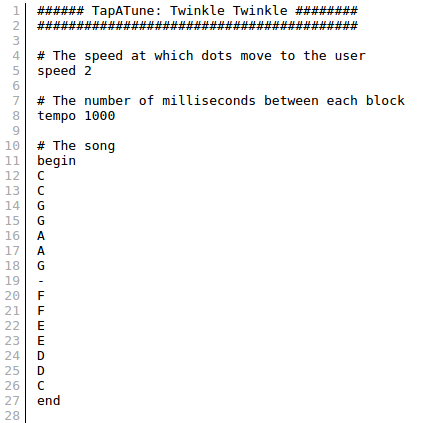
\includegraphics[width=15em]{song}
  \captionsetup{justification=justified,singlelinecheck=false}
  \caption*{\fontsize{9}{9}\selectfont \textbf{Figure 2.} The contents of the Twinkle Twinkle song, which is read into our game. The first few lines of the file detail how fast the dots move on the screen and the tempo of the song, and then the `begin' and `end' keywords signal when to start reading in the notes. }
\end{figure}

\subsection{Design}

When planning the design of our game, we drew lots of parallels with the well-known game \emph{Guitar Hero}, and this helped us with setting realistic goals and milestones based on the various features of the game. We split into groups of two to do some preliminary research on how to implement sound and GUIs in C. Notably, progress in the graphics area was made much faster than progress in the sound area, as we were able to quickly code a user interface for our game. One member of the group also was quickly able to setup a program which read user input through the keyboard. This was important as it corresponded to the user's pressing of the GUI's buttons, each of which represented a different guitar string.

\vspace{0.2in}

As is good practice in C, we created a header file, which consisted of numerous constants, enumerations, structs, and function definitions. We created a main game object, which we passed around to all methods as a pointer. This gave us the most flexibility in terms of accessing all the game properties, without needing to make any variables global. We were able to code the graphics within a few days, after which we started to make tests on the graphics, while we waited to integrate the sound component of the extension.

\vspace{0.2in}

Once we were able to figure out how to play a sound, using the SDL Mixer platform, the ball was rolling. We extended our progress to have the program play multiple sound effects at once, to create a more realistic interpretation of pressing several notes. We were now able to read sounds from a file, read user input, and integrate both into our advanced graphics. \textbf{Figure 3} shows the process of listening to a keypress event, and reacting by increasing the score.

\subsection{Challenges}

\begin{itemize}

\item Lag - The GUI that we coded initially encountered a tremendous amount of lag as the buttons were falling down the screen. To fix this, we optimised the graphics so that the buttons would immediately free memory after their termination. This also improved lag time.

\item Playing Multiple Sounds - This challenge was fixed through copious amounts of research. We were trying to play sounds simultaneously along with the GUI, so we could also respond to the pressing of multiple buttons. This was finally accomplished after thorough research and extensive development.

\end{itemize}

\subsection{Testing}

To be written.

\section{Reflections}

\subsection{Group Reflection}

This group project served as a true test to both our individual programming abilities and our teamwork skills. Throughout the duration of the project, it was essential to maintain good communication, and effectively distribute work. Overall, it is our pleasure to say that the group dynamic was exceptional throughout the duration of the project, and this resulted in completing the first three parts of the project at excellent pace, along with creating an excellent extension.

\vspace{0.2in}

\textbf{Communication}. Keeping in contact as a group was vital and something we prided ourselves on doing constantly. Facebook was the main form of communication, where we were able to schedule events that corresponded to group meetings and code sessions. This ensured that all members were prompt and present to put their best foot forward towards all of the group's endeavours. The code was shared through GitLab, and at first, there were numerous conflicts with merging. However, we scheduled meetings specifically to address the logistics of pushing code to the repository, which included pulling and merging calls and the protocol for appropriate Git commits.

\vspace{0.2in}

\textbf{Version Control}. We prided ourselves on using multiple branches in our Git repository. This ensured that different members could push to different branches without confusion, and this would better organize our code. Helpful commit messages ensured that when it came time to merge our individual branches to the master, this process would be quick, and not take up time that was meant for coding. \textbf{Figure 4} shows our overall workflow in branches for the extension of the project.

\vspace{0.2in}

\textbf{Splitting the work}. For the most part, this was done really well. Just as a proper code format was expected by the group, so too was a proper written format for the checkpoint and the report. The code, from the emulator to the extension, was split very well and we would not change anything with that. We are happy with the group dynamic, as is also seen from the individual reflections.

\subsection{Individual Reflections}

\begin{myquote}
``Doing this group project was definitely the most challenging - and, in turn, the most rewarding - experience of my first year at Imperial. While we had a spec to follow while creating the emulator and assembler, the extension truly tested our creativity and programming abilities. There was never a time when the project came easy to us, but there never were any challenges that the group could not overcome.
\\Reflecting on my own performance, I am very satisfied with my contributions to the group. I was in charge of Part III, writing GPIO and getting the LED to turn on in the Raspberry Pi. Additionally, as the strongest writer in the group, I had a key part in writing both the checkpoint and the report. Of course, in every part of the project, the work did not fall on just one person. I felt that the group was able to collaborate really well on all parts, as I coded certain instructions in both the assembler and emulator, as well.
\\If I could make one change to the whole process, I would definitely focus on XXXXXXXXXXXX. Otherwise, this project - especially the extension - brought out the best in my programming abilities and was integral to my first year at Imperial!"
\end{myquote}
\rightline{{\rm --- Shravan Nageswaran}}


\begin{myquote}\noindent
``I am very happy with the performance of my entire group in this project, and I have really enjoyed the challenge. It has been exciting and rewarding to be the group leader and I believe that I have managed the group well throughout. Having a lot of experience in programming has proved very useful during this project, and it meant that I was able to assist my group in the more complicated aspects to the C language. One aspect of the WebPA assessment that I am most proud of is being able to point other people in the right direction when they are struggling with coding - especially when it is a segmentation fault!
\\Reflecting on my progress throughout, I think that I made a slower start to Part I than I had hoped. It took a few days for all of us to get a full understanding of the requirements of the emulator, and the hardest part of the whole project in my opinion, was the initial setup of the emulator, which involved reading in the binary file and loading in the instructions into the \emph{pipeline}. I felt a lot more comfortable after that, and we were able to make much better progress are overcoming this initial hurdle.
\\In the future, if I were to repeat this project, I would have probably started out differently. Instead of trying to understand the  specification in its entirety, I would break down the first part and get straight to programming the binary file reader. That way, we'd be in a better position to continue and work systematically. Other than that, I can't fault anything else in our group and I am extremely happy with the finished products!"
\end{myquote}
\rightline{{\rm --- Jason Lipowicz}}


\begin{myquote}
``Overall, working in this group has been enjoyable and challenging at the same time. While the group dynamic has been outstanding, there were situations where the communication between the group members could have been better. At one point two members of the group worked on the same function in the same file which resulted in many merge conflicts, which then took a long time to solve. However, this was a good learning experience for all of us in terms of both communication and using gitlab appropriately. There were also multiple disagreements on how to implement certain functions as well as extension ideas, but we were always able to find compromises.
\\This has been my first programming group project, which has proved to be a great learning experience.  I am very grateful to other members of my group for patiently helping me overcome the challenges that I faced, which made me a better C programmer. Although I believe that I have put a lot of effort into this project, I admittedly had a slower start than other members of the group, but I hope that I have managed to compensate for that by working harder for the assembler and extension parts of the project. The increase in my WebPA assessment grade has shown to me that other group members value the extra effort that I've put in, which motivated me further to work even harder to further improve our extension."
\end{myquote}
\rightline{{\rm --- Alexandr Zakon}}


\begin{myquote}
``This project gave us the freedom to develop and implement our own ideas which motivated us to advance at a faster pace until its successful completion.
\\
Reflecting on my progress, I believe that once I have passed the beginning and gained a deeper understanding of the C programming language I could really enjoy solving problems and realising my vision through the development of the project, and especially the extension. The primary stages took more time to complete. At about the midpoint of the project, after completing the emulator, I became more eager to succeed and this was driven by seeing my vision take shape. This is also reflected in the feedback I received from my group members in WebPA. I contributed to all parts of the project and enjoyed understanding the computer memory through C and being in charge of memory management.
\\
Reflecting on our performance as a group, I am very satisfied with our work and the dynamics of our group. We communicated well, which I felt made us a strong group and allowed us all to contribute the most. This project was very challenging, though rewarding and enjoyable at the same time.
\\
If I could change one thing in the process, I would split the first parts into smaller tasks to allow a faster completion and have more time to develop the extension."

\end{myquote}
\rightline{{\rm --- Boaz Francis}}


\section{Conclusion}

The ARM project and extension have definitely been challenging, but, with the help of our fellow group members, we feel that we have learnt and achieved a lot from this experience.

\vspace{0.2in}

We believe our efforts not only showcase themselves in the first three parts, but equally in the extension, as well. The depth and nuances of our game required immense effort, efficient communication, and proficient coding amongst our group members, and, while our project is not quite finished, we are pleased with our current work.

\vspace{0.2in}

Overall, we were satisfied with our group experience, and we feel that is reflected in our product.

\end{document}
